% Chapter X

\chapter{DSMC WITH SPIN - MCWF} % Chapter title

\label{ch:dsmcmcwf} % For referencing the chapter elsewhere, use \autoref{ch:dsmcmcwf} 

I guess I need to talk about the MCWF method here, this could be difficult.

%---------------------------------------------------------------------------------------
\section{Single Atom Spin Flips}

Just like we did with the Ehrenfest method in section \ref{sec:EhrenfestSingleAtom} we can begin by simulating the a spin flip of a single atom in a Majorana type trap. 
To make the comparison between the two methods fair we will again use the same magnetic field, $\mathbf{B} = (B_x,0,B_z'z)$, with $B_x=1\,\mu\mathrm{T}$ and $B_z'=2.5\,\mathrm{Tm}^{-1}$.
Our rubidium 87 atom will also have the same initial conditions, $z=-5\,\mu\mathrm{m}$ and zero initial velocity, $v_z=0\,\mathrm{ms}^{-1}$.
Finally we will use the same simulation time step, $\Delta t = 0.1\,\mu\mathrm{s}$.
The only difference here is that we must average the result over a large number of simulations, in this case we have run $10^5$ independent simulations.

\begin{figure}
\hspace{-8em}
\makebox[1.8\linewidth][l]{%
\centering
\subfloat[Co-rotating frame spins]{\label{fig:mcwfMajoranaSpin}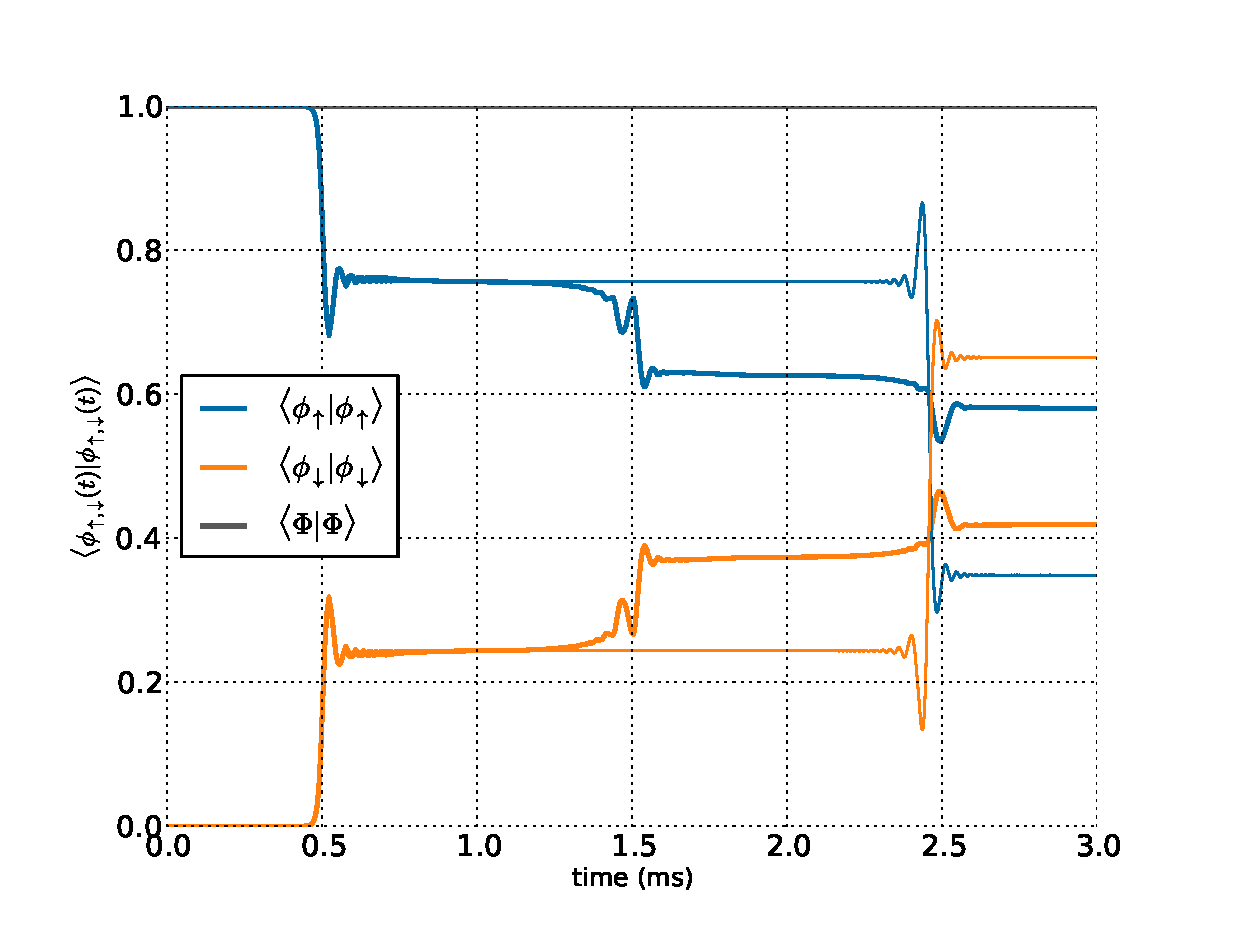
\includegraphics[width=0.525\textwidth]{gfx/MCWF/mcwfMajoranaSpin}}\quad
\subfloat[Position and velocity]{\label{fig:mcwfMajoranaTrajectory}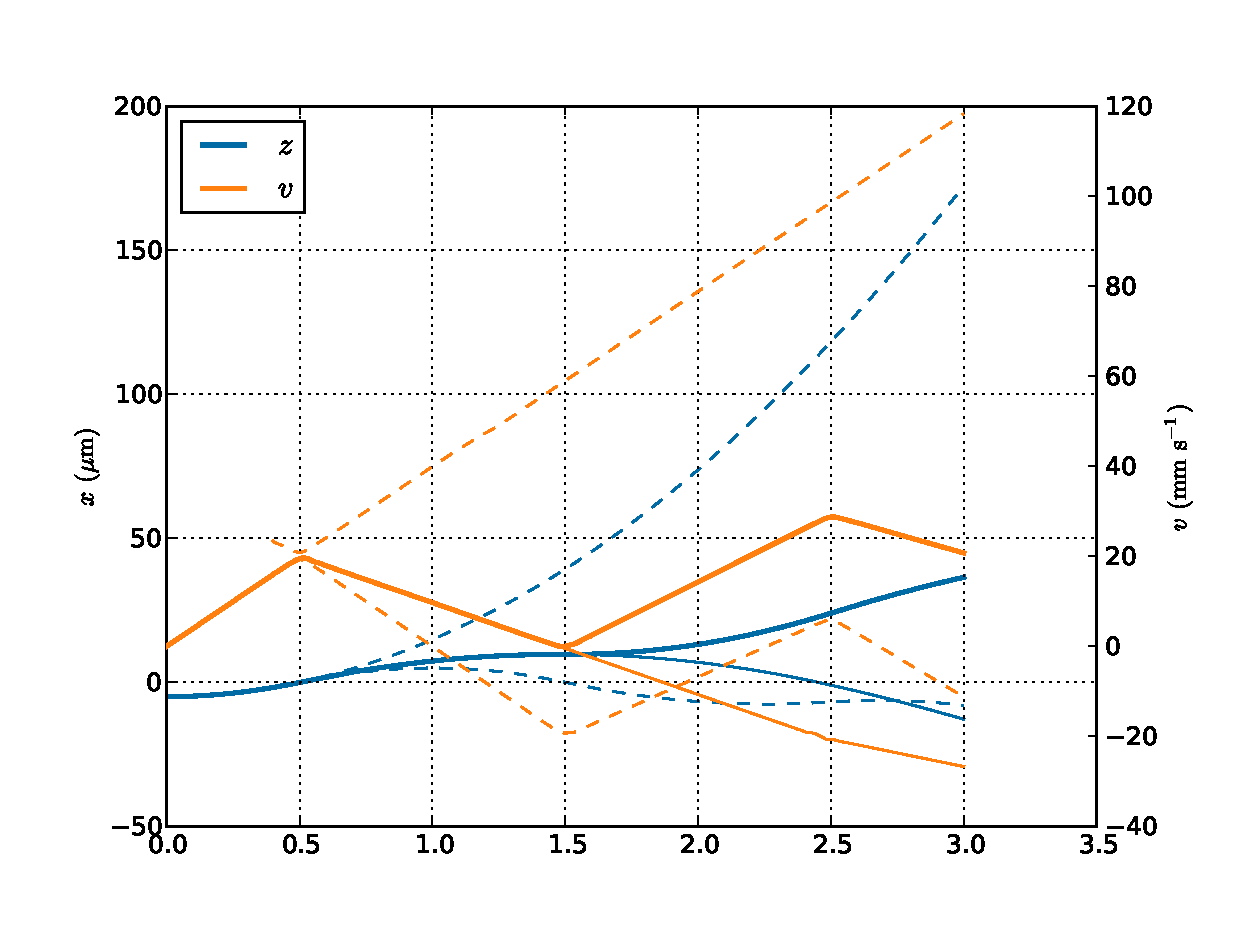
\includegraphics[width=0.525\textwidth]{gfx/MCWF/mcwfMajoranaTrajectory}}\quad
\subfloat[Energy]{\label{fig:mcwfMajoranaEnergy}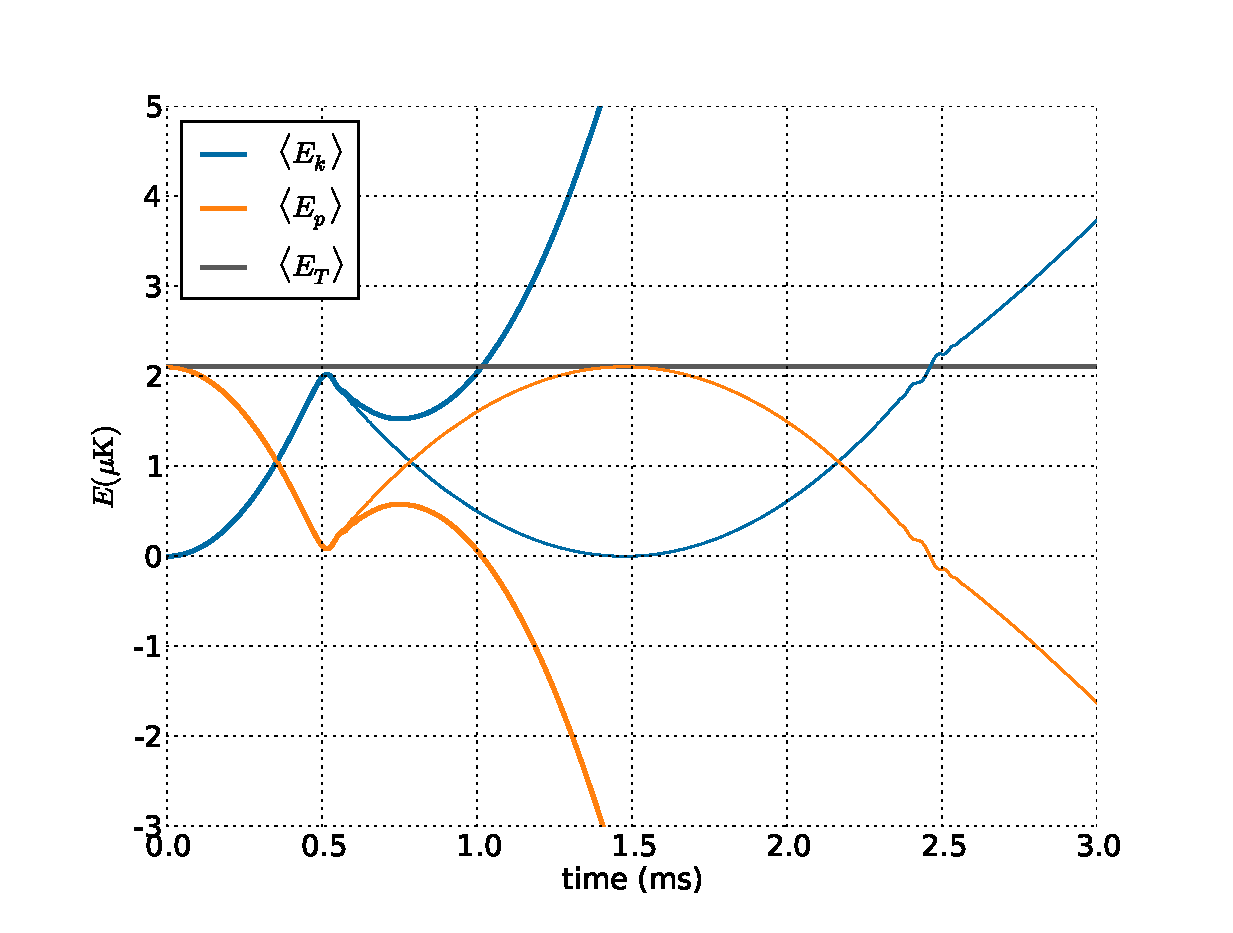
\includegraphics[width=0.525\textwidth]{gfx/MCWF/mcwfMajoranaEnergy}}%
}
\caption{No flip and flip in the same simulation mcwf.}\label{fig:mcwfFlip}
\end{figure}

At last, in figure \ref{fig:mcwfFlip} we have some convincing proof of the failure of the Ehrenfest method.
First let's get the boring stuff out of the way.
Figure \ref{fig:mcwfMajoranaSpin} illustrates that the MCWF method conserves probability, similarly figure \ref{fig:mcwfMajoranaEnergy} shows the energy conservation of the method.
Now let's compare the differences between the Ehrenfest and MCWF methods.
We'll start by comparing the wavefunction evolution depicted in figure \ref{fig:mcwfMajoranaSpin}.
Here we see the two methods agree perfectly for the first magnetic field minimum crossing.
However, at around $1.5\,\mathrm{ms}$ we see the MCWF method make, what looks to be another spin flip, and then another at $2.5\,\mathrm{ms}$.
How can this be?
What is it that causes the particles in the MCWF method to experience an extra spin flip?
This questions is most clearly illustrated in figure \ref{fig:mcwfMajoranaTrajectory}.
The bold lines indicate the averaged trajectories of the MCWF particles.
Again up until the $1.5\,\mathrm{ms}$ mark the two approaches (Ehrenfest and MCWF) agree exactly.
So what is it that happens at $1.5\,\mathrm{ms}$ that causes this deviation?
Consider the trajectories shown by the dashed lines.
These lines represent the average trajectories of all the particles who are considered to be in a trapped state.
Conversely the dash-dotted lines are the untapped state.
While the average of these two trajectories produces the same result as the Ehrenfest method (as we might expect), the physical path taken by the particles is completely different.
So the reason for the apparent extra spin flip at $1.5\,\mathrm{ms}$ is due to the extra crossing of the field minimum experienced by the particles that remain in the trapped state.
So what happens in the Ehrenfest simulation?
What is it that produces its failure?
The Ehrenfest method will move particle along the trajectory described by the average force.
At $0.5\,\mathrm{ms}$ after the first crossing of the field minimum the particle experiences a partial flip.
Since the particle is moved with the average force the trapping force of the particle is now weaker and it is effectively trapped in a looser magnetic field.
While on average this may be a reasonable way to think about the problem, we have already seen that it does not produce the correct dynamics for particles moving in a simple one-dimensional trap.

How does this result explain the disagreement of the Ehrenfest method with the test done in section \ref{sec:EhrenfestQuad}?
When a particle experiences a partial flip the Ehrenfest method will then subject it to a weaker trapping force, essentially loosening or widening the trapping potential.
So in figure \ref{fig?} as the particles of the gas slowly begin to tip over, from the cumulative effect of many partial flips, the gas begins to unnaturally widen.
As a result the calculated temperature is higher than what one would physically expect.
In practice we know that an atom is either in a trapped state or an untrapped state (not partially in both).
So a real trapped gas that is subjected to Majorana spin flips should not display a widening due to the weakening trapping potential, it should only exhibit atom loss due to the fully flipped atoms leaving the trap\footnote{Of course this will also result in a widening of the trap due to the heating effect cause by the selective removal of the least energetic particles.}.

So why does the Ehrenfest method seem to work for the Ioffe Pritchard trap?
We do not expect atoms in the IP trap to undergo any kind of spin flip.
The geometry of the trap is such that the rate of change of the magnetic field direction is always (JUSTIFY?) less than the Larmor precession rate.
So the particles in the simulation shown in figure \ref{fig:ehrenfestIP} are always subjected to the full trapping potential.

%----------------------------------------------------------------------------------------

\section{Full Gas Simulations}

Content

%------------------------------------------------

\subsection{Ioffe Pritchard Trap}

Content

%------------------------------------------------

\subsection{Quadrupole Trap}

Content